
%----------------------------------------------------------------------------------------
%	PACKAGES AND OTHER DOCUMENT CONFIGURATIONS
%----------------------------------------------------------------------------------------

\documentclass[twoside,11pt,a4paper,openright]{Thesis} % The default font size and one-sided printing (no margin offsets)[11pt, oneside]

\graphicspath{{Pictures/}} % Specifies the directory where pictures are stored


\usepackage[square, numbers, comma, sort&compress]{natbib} % Use the natbib reference package - read up on this to edit the reference style; if you want text (e.g. Smith et al., 2012) for the in-text references (instead of numbers), remove 'numbers'
\usepackage{eurosym}

\hypersetup{urlcolor=blue, colorlinks=true} % Colors hyperlinks in blue - change to black if annoying
\title{\ttitle} % Defines the thesis title - don't touch this

\begin{document}

\frontmatter % Use roman page numbering style (i, ii, iii, iv...) for the pre-content pages

\setstretch{1.3} % Line spacing of 1.3

% Define the page headers using the FancyHdr package and set up for one-sided printing
\fancyhead{} % Clears all page headers and footers
\rhead{\thepage} % Sets the right side header to show the page number
\lhead{} % Clears the left side page header

\pagestyle{fancy} % Finally, use the "fancy" page style to implement the FancyHdr headers

\newcommand{\HRule}{\rule{\linewidth}{0.5mm}} % New command to make the lines in the title page

% PDF meta-data
\hypersetup{pdftitle={\ttitle}}
\hypersetup{pdfsubject=\subjectname}
\hypersetup{pdfauthor=\authornames}
\hypersetup{pdfkeywords=\keywordnames}

%----------------------------------------------------------------------------------------
%	TITLE PAGE
%----------------------------------------------------------------------------------------

\begin{titlepage}
\begin{center}

%\textsc{\LARGE \univname}\\[0.5cm] % University name
\textsc{\LARGE Research Internship Report}\\[0.1cm]
 {\Large 25/04/2016  $\sim$  25/09/2015}\\[0.5cm] % Thesis type

\HRule \\[0.4cm] % Horizontal line
{\textbf{\huge  Deep Learning and Reality Gap}}\\[0cm] % Thesis title
\HRule \\[2.5cm] % Horizontal line

\begin{figure}[htbp]
	\centering
		
\includegraphics[width=\textwidth,height=\textheight,keepaspectratio]{Figures/logo.png}
\end{figure}
\vspace{2.2cm}

\emph{\LARGE Author:}\\[0.2cm]
{\LARGE\authornames}\\[2.8cm]% Author name - remove the \href bracket to remove the link


%\emph{\Large Industrial Supervisor:} \\
%{\supname} \\% Supervisor name - remove the \href bracket to remove the link
%{\supnamex} \\% Supervisor name - remove the \href bracket to remove the link
%{\supnamexx}\\[0.5cm] % Supervisor name - remove the \href bracket to remove the link

%\emph{\Large Academic Supervisor:}\\
%{\examname} \\[2cm]% Author name - remove the \href bracket to remove the link

\large \textit{A report submitted in fulfilment of the requirements\\ for the degree of Master in Computer Science}\\[0.3cm] % University requirement text
\textit{at}\\[0.4cm]
{\Large Telecom Paristech}\\[2.5cm] % Research group name and department name

{\large \today}\\[4cm] % Date
%\includegraphics{Logo} % University/department logo - uncomment to place it

\vfill
\end{center}
\cleardoublepage
\end{titlepage}

%----------------------------------------------------------------------------------------
%	SUPERVISORS
%----------------------------------------------------------------------------------------
\setstretch{1.5} % Reset the line-spacing to 1.5 for body text (if it has changed)

\supervisors{\addtocontents{toc}{\vspace{1em}} % Add a gap in the Contents, for aesthetics
\vspace{1cm}

\emph{\Large Scientific Supervisors:}\\[0.5cm]
{Michele SEBAG} \\% Supervisor name - remove the \href bracket to remove the link
Head of Équipe A-O - LRI\\
Tel : 01.69.15.42.33\qquad E-mail : \href{mailto:sebag@lro.fr}{sebag@lri.fr}\\[0.3cm]

\emph{\Large Academic Supervisor:}\\[0.5cm]
{Albert BIFET} \\
Associate Professor in Big Data\\
Télécom ParisTech\\
\qquad E-mail : \href{mailto:albert.bifet@gmail.com}{albert.bifet@gmail.com}
}

%----------------------------------------------------------------------------------------
%	ACKNOWLEDGEMENTS
%----------------------------------------------------------------------------------------

\cleardoublepage

\acknowledgements{\addtocontents{toc}{\vspace{1em}} % Add a gap in the Contents, for aesthetics
The internship opportunity I had with TAO group was a great chance for learning and for research experience. It’s here at TAO I strengthened my willing to future research careers. Therefore, I consider myself as a very lucky individual as I was provided with an opportunity to be a part of it. I am sincerely grateful for having a chance to meet so many wonderful people who led me through this five-month internship.

First and foremost, I would like to express my sincere gratitude to my supervisor Mme. Michele SEBAG, for the continuous support of my internship, for her patience, motivation, and immense knowledge. Her guidance helped me in all the time of research and writing of this report. I could not have imagined having a better superadvisor and mentor for my internship.

My sincere thanks also goes to M. Gaetan Marceau Caron, who provided me his knowledge and experience and precious time, only with his help I can get better work enviroment.

Last but not the least, I would like to thank all the TAO team members. Thank you for the fabulous leisure time we had together!
}

%----------------------------------------------------------------------------------------
%	LIST OF CONTENTS/FIGURES/TABLES PAGES
%----------------------------------------------------------------------------------------
\pagebreak

\pagestyle{fancy} % The page style headers have been "empty" all this time, now use the "fancy" headers as defined before to bring them back

\lhead{\emph{Contents}} % Set the left side page header to "Contents"
\tableofcontents % Write out the Table of Contents

\addtocontents{toc}{\vspace{1em}} % Add a gap in the Contents, for aesthetics

\lhead{\emph{List of Figures}} % Set the left side page header to "List of Figures"
\listoffigures % Write out the List of Figures

%----------------------------------------------------------------------------------------
%	THESIS CONTENT - CHAPTERS
%----------------------------------------------------------------------------------------

\addtocontents{toc}{\vspace{1em}} % Add a gap in the Contents, for aesthetics

\mainmatter % Begin numeric (1,2,3...) page numbering

\setstretch{1.5} % Return the line spacing back to 1.5

\pagestyle{fancy} % Return the page headers back to the "fancy" style

% Include the chapters of the thesis as separate files from the Chapters folder
% Uncomment the lines as you write the chapters

% Chapter 1

\chapter{Introduction} % Main chapter title

\label{Chapter1} % For referencing the chapter elsewhere, use \ref{Chapter1}

\lhead{Chapter 1. \emph{Introduction}} % This is for the header on each page - perhaps a shortened title

%----------------------------------------------------------------------------------------

Deep learning is part of a broader family of machine learning methods based on learning representations of data. In the recent years, Artificial Neural Nerwork has achieved a success in the domains like Computer Vision, Natural Language Processing. 

Research in this area attempts to make better representations and create models to learn these representations from large-scale unlabeled data. Some of the representations are inspired by advances in neuroscience and are loosely based on interpretation of information processing and communication patterns in a nervous system, such as neural coding which attempts to define a relationship between various stimuli and associated neuronal responses in the brain.\cite{olshausen1996emergence}

In the field of neuroscience, the data of electroencephlogram data(EEG Data) are being used in the brain computer interface(BCI), for example, using the EEG data to control the wheelchair or the gamestick. But they are facing the problem that the EEG data has a high variability problem. The data is not only depends on the subject, but also depends on the session. Which is to say that the EEG data collected in the morning and in the evening from the same subject is different. So it asks to train a model depends on a subject and then to adjust the model for different session.

Domain Adaptation\cite{bridle1990recnorm}\cite{ben2010theory} is a field associated with machine learning and transfer learning. This scenario arises when we aim at learning from a source data distribution a well performing model on a different (but related) target data distribution. For instance, one of the tasks of the common spam filtering problem consists in adapting a model from one user (the source distribution) to a new one who receives significantly different emails (the target distribution). Note that, when more than one source distribution is available the problem is referred to as multi-source domain adaptation.\cite{crammer2008learning}

In this internship, I work under the supervision of Dr. Michele Sebag and Dr. Gaetan Marceau Caron at Laboratoire de Recherche en Informatique (LRI), Gif-sur-Yvette, France. We aim at using domain adaptation to eliminate the variability of the EEG data. 


%-----------------------------------------------------------------------------------------
\section{Outline}
In the first part( \autoref{Chapter2}) the contexte and the objectif of this internship will be introduced, the detail of EEG data, domain adaptation will be explained.

\autoref{Chapter3} will show the state of the art on the field of deep learning or more presicely the domain adaptation.

The following chapter( \autoref{Chapter4}) focuses on the framework of this internship, the program I used to train the model.

\autoref{Chapter5} will give you the experiments I have done and the results achieved. Some comments will also follow the results.

The final \autoref{Chapter6} will be the discussion of the experiments results of using domain adaptation on the EEG data to eliminate the variability problem. Then the perspective of the subject will be given. %introduction
% Chapter 2

\chapter{Context and Objective} % Main chapter title

\label{Chapter2} % For referencing the chapter elsewhere, use \ref{Chapter2}

\lhead{Chapter 2. \emph{Context and Objective}} % This is for the header on each page - perhaps a shortened title
In this chapter, I will first introduce the context of this internship which is the Brain Computer Interface (BCI) and the new deep learning technique Domain Adaptation. From the problems identified for the EEG data, we propose the approach by using Domain Adaptation to eliminate the variabilty problem in the EEG data.

%----------------------------------------------------------------------------------------

\section{Context}


\subsection{BCI}{Brain Computer Interface}
Brain-computer interface is a method of communication based on neural activity generated by the brain and is independent of its normal output pathways of peripheral nerves and muscles. The neural activity used in BCI can be recorded using invasive or noninvasive techniques. The goal of BCI is not to determine a person's intent by eavesdropping on brain activity, but rather to provide a new channel of output for the brain that requires voluntary adaptive control by the user.\cite{wolpaw2000brain} The potential of BCI systems for helping handicapped people is obvious, the wheelchair controled by EEG signal is shown at \fref{fig:wheelchair}. There are several computer interfaces designed for disabled people.\cite{wickelgren2003brain} Most of these systems, however, require some sort of reliable muscular control such as neck, head, eyes, or other facial muscles. It is important to note that although requiring only neural activity, BCI utilizes neural activity generated voluntarily by the user. Interfaces based on involuntary neural activity, such as those generated during an epileptic seizure, utilize many of the same components and principles as BCI, but are not included in this field. BCI systems, therefore, are especially useful for severely disabled, or locked-in, individuals with no reliable muscular control to interact with their surroundings.

\begin{figure}[htbp]
	\centering
	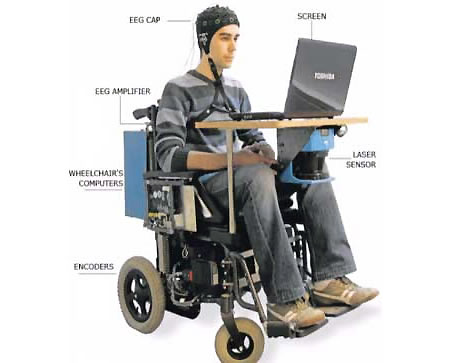
\includegraphics[width=10cm]{Figures/wheelchair.jpg}
	\caption[A wheelchair controled by EEG signal]{A wheelchair controled by EEG signal}
	\label{fig:wheelchair}
\end{figure}

But there's a main limitation for BCI is that the EEG data have a high inter-variability and intra-variability. EEG data are highly dependent on subject, so it requires to train the BCI on each subject. Also, it's highly dependent on session, EEG collected are varies from different time(like morning and evening), and even during a same work session, so it also requires to train on each subject for each session, which is difficult to realize and redundant. Thus we should find an approach to eliminate the subject-independent and session independent problem of EEG data.

\subsection{Domain Adaptation}
Top-performing deep architectures are trained on massive amounts of labeled data. In the absence of labeled data for a certain task, domain adaptation often provides an attractive option given that labeled data of similar nature but from a different domain (e.g. synthetic images) are available. The paper by [Ganin et al. 2015]\cite{ganin2014unsupervised} propose a new approach to domain adaptation in deep architectures that can be trained on large amount of labeled data from the source domain and large amount of unlabeled data from the target domain (no labeled target domain data is necessary).

As the training progresses, the approach promotes the emergence of “deep” features that are
\begin{enumerate}
	\item Discriminative for the main learning task on the source domain
	\item Invariant with respect to the shift between the domains.
\end{enumerate} 
The paper\cite{ganin2014unsupervised} shows that this adaptation behavior can be achieved in almost any feed-forward model by augmenting it with few standard layers and a simple new \textbf{gradient reversal layer}. The resulting augmented architecture can be trained using standard back-propagation. Overall, the approach can be implemented with little effort using any of the deep-learning packages. The method performs very well in a series of image classification experiments, achieving adaptation effect in the presence of big domain shifts and outperforming previous state-of-the-art on Office datasets.

\begin{figure}[htbp]
	\centering
	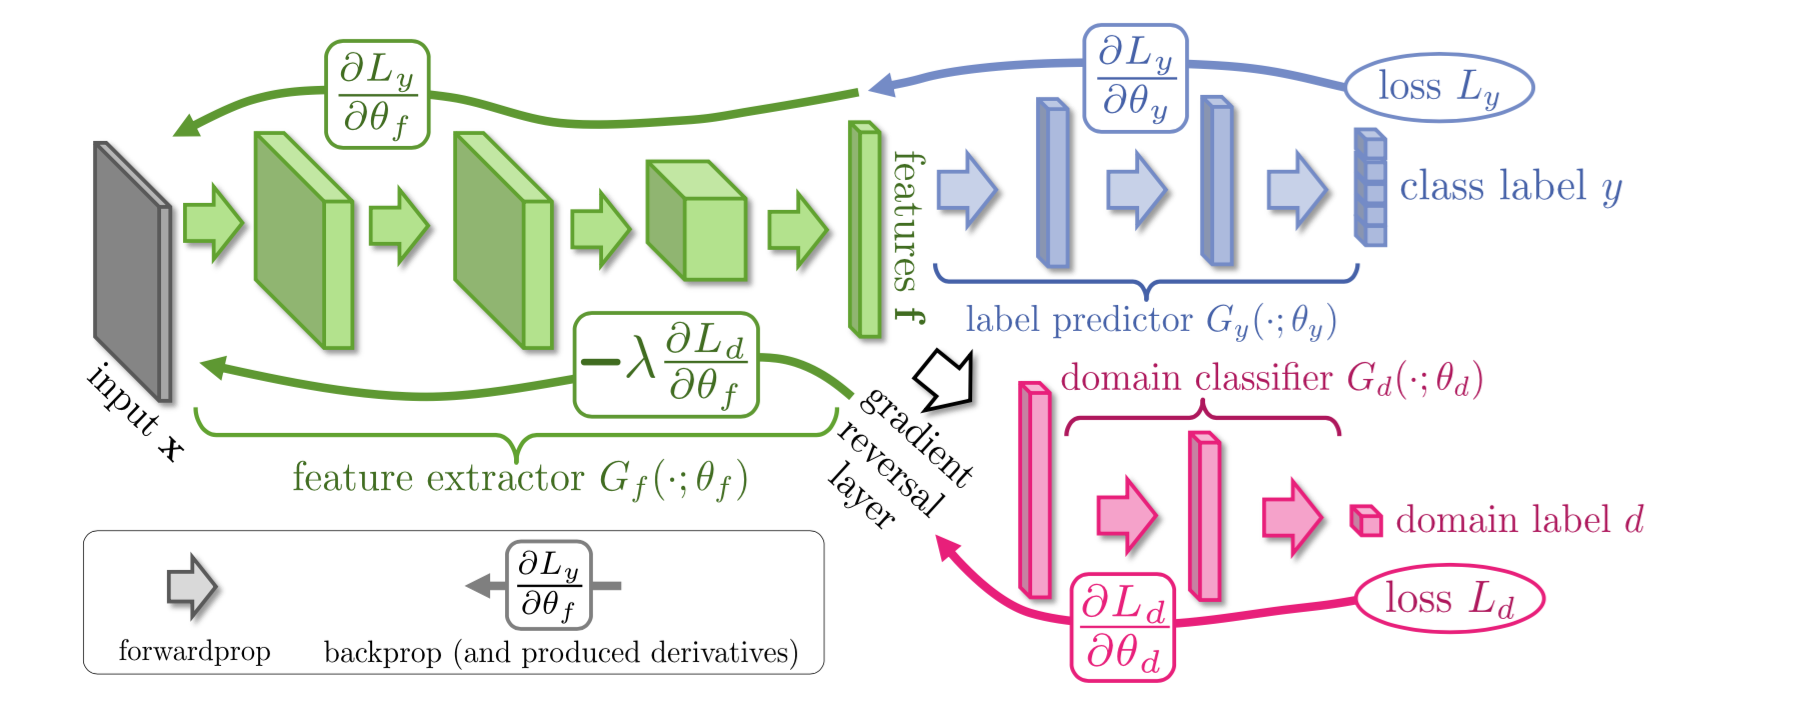
\includegraphics[width=15cm]{Figures/domainadaptation.png}
	\caption[Domain Adaptation Model Architecture]{Domain Adaptation Model Architecture}
	\label{fig:domainadaptation}
\end{figure}

This method involves two domains, the source domain and the target domain.  For example, the source domain can be MNIST dataset (handwritten digit database) and the target domain can be the SVHN dataset (The Street View House Numbers). Formally, the source is described through a training set, made of (instance, label) pairs:
\[ \mathcal{ S} = {(x_{i},y_{i}), x_{i} \in X, y_{i} \in Y, i \in [1,n]}  \]
where \textit{X} is the instance space (e.g. the vectors of pixel values) and \textit{Y} is the label space (e.g. the digit numbers). The target is described through a test set made of instances:
\[ \mathcal{T} = x'_{i}, x'_{i} \in X, i \in [1,n] \]
The general goal is to build a classifier \textit{h} for the source domain and for the target domain \textbf{without} gathering the target doamin labels.

The paper has proposed a model for the domain adaptation as \fref{fig:domainadaptation}. The proposed architecture includes a deep feature extractor (green) and a deep label predictor (blue), which together form a standard feed-forward architecture. Unsupervised domain adaptation is achieved by adding a domain classifier (red) connected to the feature extractor via a gradient reversal layer that multiplies the gradient by a certain negative constant during the backpropagationbased training. Otherwise, the training proceeds in a standard way and minimizes the label prediction loss (for source examples) and the domain classification loss (for all samples). Gradient reversal ensures that the feature distributions over the two domains are made similar (as indistinguishable as possible for the domain classifier), thus resulting in the domain-invariant features.

During the learning stage, we aim to minimize the label prediction loss on the annotated part (i.e. the source part) of the training set, and the parameters of both the feature extractor and the label predictor are thus optimized in order to minimize the empirical loss for the source domain samples. This ensures the discriminativeness of the features \textbf{f} and the overall good prediction performance of the combination of the feature extractor and the label predictor on the source domain. At the same time, we want to make the features \textbf{f} domain-invariant which is we want the representation of the two domains to be similar.

At training time, in order to obtain domain-invariant features, we seek the parameters of the feature mapping that maximize the loss of the domain classifier (by making the two feature distributions as similar as possible), while simultaneously seeking the parameters of the domain classifier that minimize the loss of the domain classifier. So as we can see, the parameter $\lambda$ of the Gradient Reversal Layer controls the trade-off between the two objectives that shape the features during learning.
%----------------------------------------------------------------------------------------

\section{Objective}
After the problem identified of the EEG data using in the BCI (high inter-variability and high intra-variability) .the objective of this internship thus is to build a subject-dependent, session-dependent representations of the EEG data. The sought representation must achieve a lossy compression of the signal to enabling the reconstruction of the brainwave data in order to further use in the BCI, besides, the representation of the signals gathered along different sessions follows the same distribution, or distribution as similar as possible. There's also a difficulty is that this reconstruction must preserve the complex spatio-temporal-frequency structure of the EEG data.




 %contexte and objectif
% Chapter 3

\chapter{State of the Art} % Main chapter title here

\label{Chapter3} % For referencing the chapter elsewhere, use \ref{Chapter3}

\lhead{Chapter 3. \emph{State of the Art}} % This is for the header on each page perhaps a shortened title
%----------------------------------------------------------------------------------------
Recently, some scientist use deep learning network on the EEG data to do the emotion recognition, also some other domain adaptation methods have been proposed over the recent years, I will list the abstract of this papers in this chapter to give you the state of the art for this subject.

\section{EEG-based emotion classification using deep belief networks}
\textbf{Abstract:}\cite{zheng2014eeg}
In recent years, there are many great successes in using deep architectures for unsupervised feature learning from data, especially for images and speech. In this paper, we introduce recent advanced deep learning models to classify two emotional categories (positive and negative) from EEG data. We train a deep belief network (DBN) with differential entropy features extracted from multichannel EEG as input. A hidden markov model (HMM) is integrated to accurately capture a more reliable emotional stage switching. We also compare the performance of the deep models to KNN, SVM and Graph regularized Extreme Learning Machine (GELM). The average accuracies of DBN-HMM, DBN, GELM, SVM, and KNN in our experiments are 87.62\%, 86.91\%, 85.67\%, 84.08\%, and 69.66\%, respectively. Our experimental results show that the DBN and DBN-HMM models improve the accuracy of EEG-based emotion classification in comparison with the state-of-the-art methods.


\section{EEG-Based Emotion Recognition Using Deep Learning Network with Principal Component Based Covariate Shift Adaptation}
\textbf{Abstract:}\cite{jirayucharoensak2014eeg}
Automatic emotion recognition is one of the most challenging tasks. To detect emotion from nonstationary EEG signals, a
sophisticated learning algorithm that can represent high-level abstraction is required. This study proposes the utilization of a deep
learning network (DLN) to discover unknown feature correlation between input signals that is crucial for the learning task.The DLN
is implemented with a stacked autoencoder (SAE) using hierarchical feature learning approach. Input features of the network are
power spectral densities of 32-channel EEG signals from 32 subjects. To alleviate overfitting problem, principal component analysis
(PCA) is applied to extract the most important components of initial input features. Furthermore, covariate shift adaptation of
the principal components is implemented to minimize the nonstationary effect of EEG signals. Experimental results show that the
DLN is capable of classifying three different levels of valence and arousal with accuracy of 49.52% and 46.03%, respectively. Principal
component based covariate shift adaptation enhances the respective classification accuracy by 5.55% and 6.53%. Moreover, DLN
provides better performance compared to SVM and naive Bayes classifiers.

\section{Domain Adaptation via Transfer Component Analysis}
\textbf{Abstract:}\cite{pan2011domain}
Automatic emotion recognition is one of the most challenging tasks. To detect emotion from nonstationary EEG signals, a
sophisticated learning algorithm that can represent high-level abstraction is required. This study proposes the utilization of a deep
learning network (DLN) to discover unknown feature correlation between input signals that is crucial for the learning task.The DLN
is implemented with a stacked autoencoder (SAE) using hierarchical feature learning approach. Input features of the network are
power spectral densities of 32-channel EEG signals from 32 subjects. To alleviate overfitting problem, principal component analysis
(PCA) is applied to extract the most important components of initial input features. Furthermore, covariate shift adaptation of
the principal components is implemented to minimize the nonstationary effect of EEG signals. Experimental results show that the
DLN is capable of classifying three different levels of valence and arousal with accuracy of 49.52% and 46.03%, respectively. Principal
component based covariate shift adaptation enhances the respective classification accuracy by 5.55% and 6.53%. Moreover, DLN
provides better performance compared to SVM and naive Bayes classifiers.

\section{Domain Adaptation for Large-Scale Sentiment Classification: A Deep Learning Approach}
\textbf{Abstract:}\cite{glorot2011domain}
The exponential increase in the availability of online reviews and recommendations makes sentiment classification an interesting topic in academic and industrial research. Reviews can span so many different domains that it is difficult to gather annotated training data for all of them. Hence, this paper studies the problem of domain adaptation for sentiment classifiers, hereby a system is trained on labeled reviews from one source domain but is meant to be deployed on another. We propose a deep learning approach which learns to extract a meaningful representation for each review in an unsupervised fashion. Sentiment classifiers trained with this high-level feature representation clearly outperform state-of-the-art methods on a benchmark composed of reviews of 4 types of Amazon products. Furthermore, this method scales well and allowed us to successfully perform domain adaptation on a larger industrial-strength dataset of 22 domains. %state of art
% Chapter 4

\chapter{Program} % Main chapter title

\label{Chapter4} % For referencing the chapter elsewhere, use \ref{Chapter4}

\lhead{Chapter 4. \emph{Program}} % This is for the header on each page - perhaps a shortened title
%----------------------------------------------------------------------------------------
\definecolor{mygreen}{rgb}{0,0.6,0}
\definecolor{mygray}{rgb}{0.9,0.9,0.9}
\definecolor{mymauve}{rgb}{0.58,0,0.82}
\definecolor{mybrown}{RGB}{178,34,34}
\lstset{language=C++,
	backgroundcolor=\color{mygray},
	numbers=left,                    % possible values are (none, left, right)
	numbersep=-8pt,                   % how far the line-numbers are from the code
	numberstyle=\tiny\color{mybrown}, % the style that is used for the line-numbers
	stepnumber=1,                    % each line will be numbered
	morekeywords={*},
	keywordstyle=\color{blue},
	stringstyle=\color{mymauve},
	commentstyle=\color{mygreen},
	morecomment=[l][\color{magenta}]{\#},
	basicstyle=\footnotesize,        % the size of the fonts that are used for the code
	keepspaces=false,                 % keeps spaces in text, useful for keeping indentation of code
	columns=flexible,
	breaklines=true
	rulesepcolor=\color{mygray},
	rulecolor=\color{mygray}
}
%----------------------------------------------------------------------------------------
The approach we proposed for this subject is using domain adaptation to eliminate the variability problem in the EEG data. In this chapter, firstly I will present the structure of EEG data we used for this internship. Then I will present the adaption of the DANN structure to our case. Thirdly is defining the criteria for our Deep Neural Network.
%----------------------------------------------------------------------------------------
\section{EEG data}
The EEG data we use is provided by Dr. Fabrizio De Vico Fallani from ICM in paris(Institut du Cerveau et de la Moelle Epinière). The EEG dataset contains 18 files. They are divided into two sessions from 9 subject. 

\begin{figure}[htbp]
	\centering
	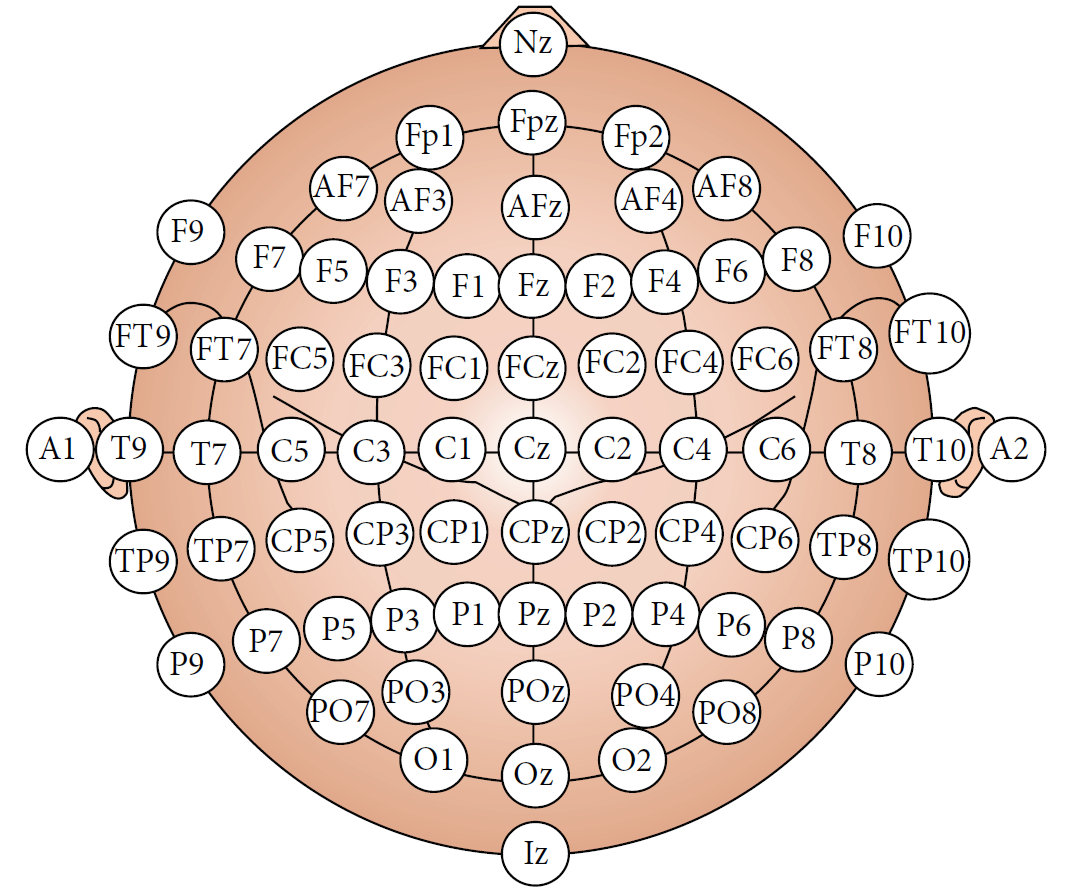
\includegraphics[width=10cm]{Figures/eegcollect.png}
	\caption[Location of the electrodes over the head of the subject]{Location of the electrodes over the head of the subject}
	\label{fig:eegcollect}
\end{figure}

The EEG signals refer to recordings of one minute during a state of no-task with closed eyes, or say "resting state". The data is collected by a helmet on the head. The helmet contains 56 electrodes all over the head, as shown in the \fref{fig:eegcollect}. The sampling frequency is equal to 200 Hz, so each file contains a matrix of 56 x 12000. 

The preprocessing for the data is normalization. I have linearly normalize the sensor values to [0,1] by:
\[ x_{i}' = \frac{x_{i}-x_{min}}{x_{max}-x_{min}} \] 
where $ x_{min} $ and $ x_{max} $ are the minimum and maximum sensor value on the session.

\section{Architecture of Dann EEG}
The principle for our adaption is that we treat session one of each subject EEG data as source domain in the Domain Adaptation, and the session two as the target domain. Once we using the DANN for training, the model will not be able to distinguish which session the input data belongs to, this is to say we can't tell the difference between session one and session two. So after reconstruction, the EEG data from two sessions become indistinguishable.

The base of our DANN is auto-encoder. An autoencoder, autoassociator or Diabolo network\cite{bengio2009learning} is an artificial neural network used for unsupervised learning of efficient codings.\cite{liou2008modeling} The aim of an autoencoder is to learn a representation (encoding) for a set of data, typically for the purpose of dimensionality reduction. Recently, the autoencoder concept has become more widely used for learning generative models of data.\cite{kingma2013auto}

Considering that the input data dimension is 56, so in the input layer and output layer of our Neural Network, the size will be 56. In this internship, which is as a first approach to solve the problem, we use a simple structure with 1 hidden layer like 56 - n -56, where n varies from 1 to 56. 

Above is the base structure of our neural network which is an auto-encoder. Then we need to add the gradient reversal layer which connected to the hidden layer. So the structure is shown in \fref{fig:eegstructure}

\begin{figure}[htbp]
	\centering
	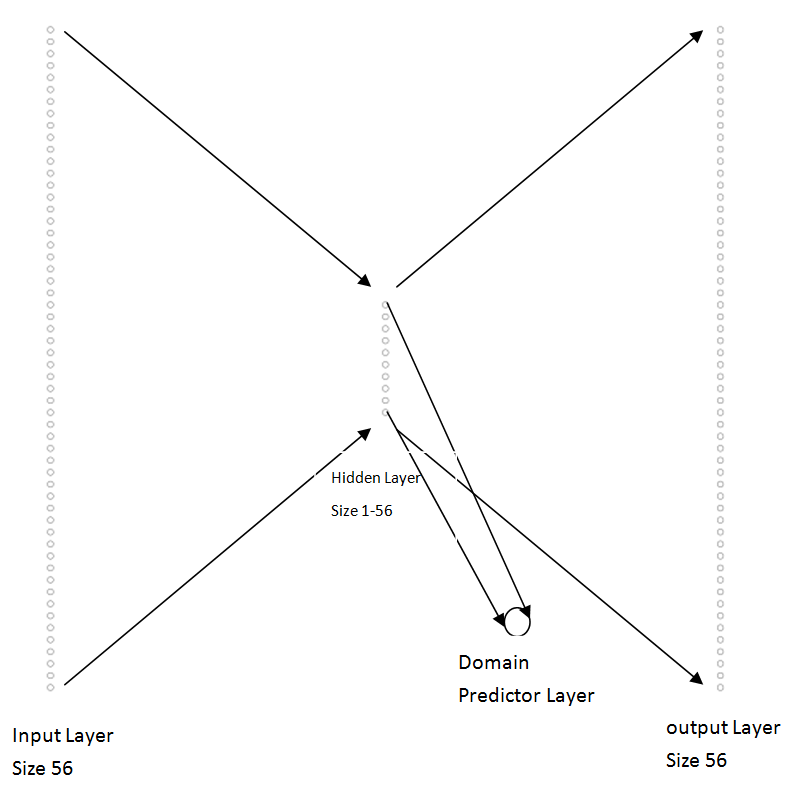
\includegraphics[width=15cm]{Figures/eegstructure.png}
	\caption[Structure of DANN for EEG data]{Structure of DANN for EEG data}
	\label{fig:eegstructure}
\end{figure}


At every neuron, the activation function will using \textbf{Sigmoid}.


\section{Criteria}
For our neural network, there are 2 purposes:
\begin{enumerate}
	\item Minimize the reconstruction error of the EEG data.
	\item Maximize the domain(session) prediction error, so that the sessions cannot be discriminated, even with the best classifier.
\end{enumerate}

Considering the requirements above, two criterion functions will be defined in the program. 

\begin{enumerate}
	\item For the reconstruction loss of EEG, we want to be able to reconstruct the initial EEG data, so we choose the MSE cost function(mean square error) like:
	\[ loss(x, \tilde{x}) = \frac{1}{n} \times \sum_{i=1}^{56}| x_{i}-\tilde{x_{i}}|^2 \]

	\item The second criterion is session-invariant. We will assess this criterion by measuring the BCE(Binary Cross Entropy) criterion of the domain(session) predictor. So the loss function will be:
	\[ loss(o, t) = -\frac{1}{n} \sum(t[i]\times \log o[i]  +  (1-t[i])\times\log (1-o[i]) \]
	where o is original prediction and t is target prediction. This criterion will give the entropy of the error, so when the result have a lot surprise, criterion will be large, otherwise the criterion will be 0.
\end{enumerate}

\section{Framework}
To realize this neural network, I have using the \textbf{Torch} framework. Torch is a scientific computing framework with wide support for machine learning algorithms that puts GPUs first. It is easy to use and efficient, thanks to an easy and fast scripting language, LuaJIT, and an underlying C/CUDA implementation.

In the torch, there's already a \textbf{gradient reversal layer} prepared to use, so we can easy connect the auto-encoder with the gradient reversal layer to build our neural network.

In the program, I have defined three separate neural network, which are:
\begin{enumerate}
	\item \textbf{Encoder}, the structure is 56 - n ($ n \in [1,56] $), this layer is used like feature extractor in the DANN, it also serves as a conpression part.
	\item \textbf{Decoder}, the structure is n - 56 ($ n \in [1,56] $), this layer is used like label predictor in the DANN, it also serves to decode the data to get the initial data.
	\item \textbf{Gradient reversal Layer}, the structure is n - 1 ($ n \in [1,56] $), this layer is used to predict which domain the instance is belonged to. With the help of negative gradient for this layer, we can maximize the error to make the two session indistinguishable. 
\end{enumerate}

Then in the training phase, the EEG data will be used as input data for Encoder, the output of Encoder will then be used as the input data of Decoder and Gradient reversal layer.

Here below is the Lua code used to build our neural network.
\begin{lstlisting}[mathescape]
	//Definition of the encoder
	featExtractor = nn.Sequential()
	featExtractor:add(nn.Linear(nInputEEG,opt.hiddenLayerUnits))
	featExtractor:add(nn.Sigmoid())
	
	//Definition of the decoder
	labelPredictor = nn.Sequential()
	labelPredictor:add(nn.Linear(opt.hiddenLayerUnits,nInputEEG))
	labelPredictor:add(nn.Sigmoid())
	
	//Definition of the domain classifier
	domainClassifier = nn.Sequential()
	domainClassifier:add(nn.GradientReversal(opt.domainLambda))
	domainClassifier:add(nn.Linear(opt.hiddenLayerUnits,1))
	domainClassifier:add(nn.Sigmoid())


\end{lstlisting} %program
% Chapter 5

\chapter{TR-069 Client} % Main chapter title

\label{Chapter5} % For referencing the chapter elsewhere, use \ref{Chapter5}

\lhead{Chapter 5. \emph{TR-069 Client}} % This is for the header on each page - perhaps a shortened title

\lstdefinestyle{DOS}
{
    backgroundcolor=\color{black},
    basicstyle=\scriptsize\color{white}\ttfamily
    numbers=none,
    numbersep=8pt,                   % how far the line-numbers are from the code
    numberstyle=\tiny\color{white}, % the style that is used for the line-numbers
    stepnumber=1                    % the step between two line-numbers. If it's 1, each line will be numbered
}
%----------------------------------------------------------------------------------------
\lstdefinestyle{C}
{
  morekeywords={export}
}
%----------------------------------------------------------------------------------------
TR-069 Client is implemented by Orange at 2008, but is a generic version for all potential devices. The first part of my internship is to make TR-069 Client for Homelive Box. To be able to provide a generic TR-069 module which is easily portable on different devices, it satisfy the following points:

\begin{itemize}
  \item Written in ANSI C
  \item Small memory footprint
  \item Provide generic API to access device specific modules
  \item Provide Makefiles to build the binary
  \item Provide system traces on module activity
\end{itemize}

On a CPE, there are two modules that are mentioned all along this document and which are responsible of
the CWMP:
\begin{itemize}
  \item \textbf{TR-069 Agent}: This agent is responsible of the CWMP sessions. It initializes them with the inform message, realizes the ACS command(s) and execute some feedback command (notably after a firmware upgrade).
  \item \textbf{TR-069 Server}: This is a small HTTP server which listens of the WAN interface for an ACS solicitation (in TR-069, it is known as “connection request”). On a valid connection request, the TR-069 server contacts the TR-069 agent for starting a CWMP session with the ACS.
\end{itemize}
%----------------------------------------------------------------------------------------
\section{Architecture of TR-069 Client}
The TR069 Generic Agent is composed of several modules and interfaces. Some modules are generic and can be ported with no modification. Other modules are platform specific (specific libraries usage, specific device API to get/set values, ...) and must implement services declared into generic interfaces.

\begin{figure}[htbp]
	\centering
		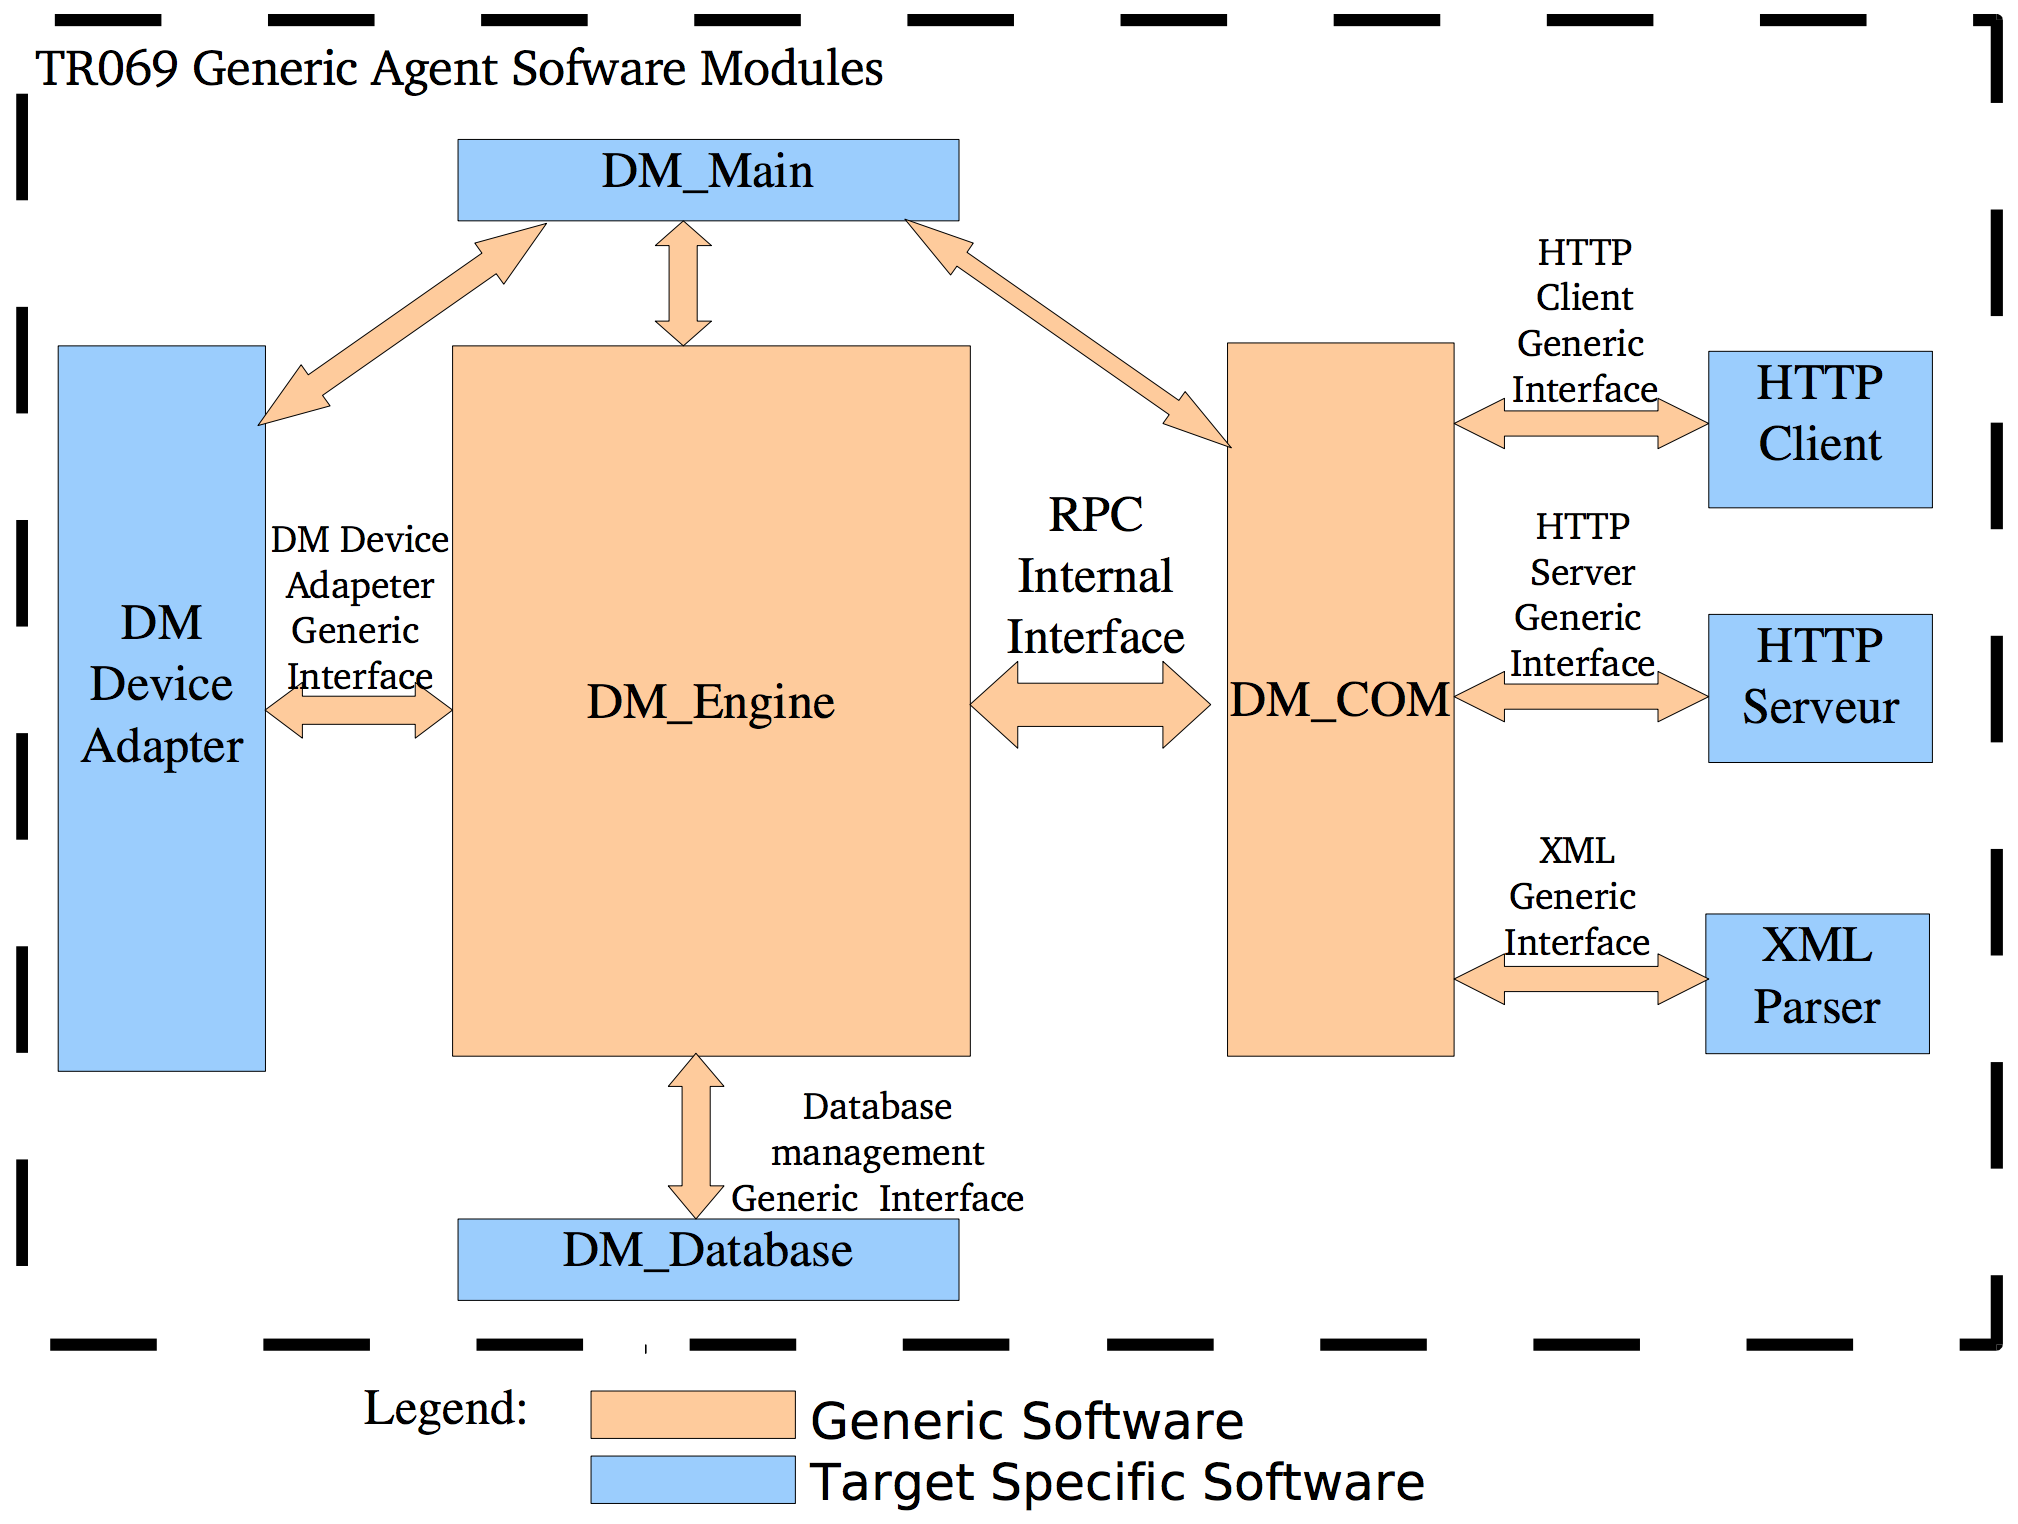
\includegraphics[width=12cm]{Figures/structuretr069.png}
	\caption[TR-069 Structure]{TR-069 Structure}
	\label{fig:tr069}
\end{figure}

For each module:
\begin{itemize}
  \item \textbf{DM\_ Engine} : In charge of the TR-069 logic,
  \item \textbf{DM\_ Com} : Handles the HTTP, SOAP and SSL Protocol with the ACS (Auto Configuration Server),
  \item \textbf{DM\_ DeviceAdapter} : Adaptation layer between the DM_Engine and the device system. It allows the implementation of the RPC commands (Get Parameter Value, Set Parameter Value, Reboot, Download, ...),
  \item \textbf{DM\_ Database} : Stores the data using an available storage solution on the device (or thanks to simple file storage),
  \item \textbf{HTTP Client} : Sets up / releases the HTTP connection with the ACS and sends / receives SOAP messages. The HTTP Client also handles SSL protocol,
  \item \textbf{HTTP SERVER} : Perform ACS Connection Request response,
  \item \textbf{XML Parser} : Decode / encode SOAP messages.
\end{itemize}

The figure below shows the file tree of the project, TR-069 Client defines all functions and APIs at each module. In consideration of easily ported to other devices, it put all target-related implementations in the folder \textit{dm\_target\_implementation}.

\begin{figure}[htbp]
	\centering
		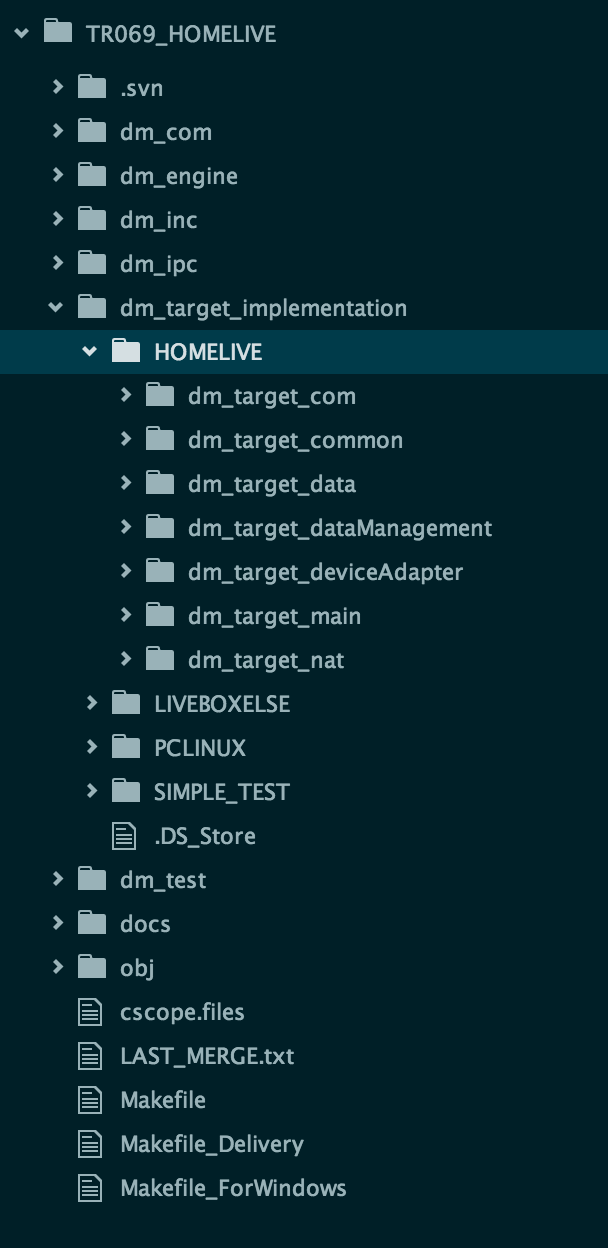
\includegraphics[width=8cm]{Figures/tr069_files.png}
	\caption[TR-069 File Tree Structure]{TR-069 File Tree Structure}
	\label{fig:tr069file}
\end{figure}

In the folder \textit{dm_taget_implementation}, different target has been defined, you can implement the APIs and Modules for different devices, and you specifie the target to compile in compilation, like:

\begin{lstlisting}[style=DOS][language=bash]
  $ make Target=TargetName TRACE_LEVEL=7 DEBUG=Y
  $ make clean Target=TargetName
\end{lstlisting}

A csv file must be created for each new platform. This CSV file describes the data model parameters used by TR069 Agent and the default values for the TR069 specifics parameters. This target dependent CSV file is stored into \\\textit{dm\_target\_implementation/MYNEWDEVICE/dm\_dm\_target\_data/dm\_csv} directory.

The CSV file is only read during the first system start up (or after a factory reset) and is used to generate the TR069
database (i.e. parameters.data and parameters.data\~{} files)

%----------------------------------------------------------------------------------------

\section{Problems and Solutions}

When ported the TR-069 Client to Homelive, we have encountered several problems before it can perfectly run on Homelive Box.

%----------------------------------------------------------------------------------------

\subsection{IP Address Error}
The first problem is IP Address Error. At every start up of the TR-069 Client, the module will have to detect the IP address of the box, and use it to build connection between STUN server and CPE. But when executing, the TR-069 client can't detect the IP address, so I have located the code which are responsible for IP detection,

\begin{lstlisting}[mathescape]
    static const char* ETH_INTERFACE = "eth0";
    struct ifaddrs *myaddrs = NULL, *ifa = NULL;
    struct sockaddr_in *s4 = NULL;
    int  status;
    /* but must be big enough for an IPv6 address (e.g. 3ffe:2fa0:1010:ca22:020a:95ff:fe8a:1cf8) */
    char buf[64];
    memset((void *) buf,  0x00, sizeof(buf));

    status = getifaddrs(&myaddrs);
    if (status == 0)
    {
       for (ifa = myaddrs; ifa != NULL; ifa = ifa->ifa_next)
       {
          if ( (ifa->ifa_addr != NULL)
             && ((ifa->ifa_flags & IFF_UP) != 0)
             && (ifa->ifa_addr->sa_family == AF_INET) )
          {
             s4 = (struct sockaddr_in *)(ifa->ifa_addr);
             if ( (inet_ntop(ifa->ifa_addr->sa_family, (void *)&(s4->sin_addr), buf, sizeof(buf)) != NULL)
                && (strcmp(ifa->ifa_name, ETH_INTERFACE)==0) )
             {
                ipAddress = strdup(buf);
                break;
             }
          }
       }
    }
\end{lstlisting}

In general, the first Internet address should be \textit{eth0}, but in Homelive Box, if you verify with command
\begin{lstlisting}[style=DOS][language=bash]
  $ ifconfig -a
\end{lstlisting}

The default Internet interface is "br-lan", which is specific in OpenWRT system, which is bridged Virtual Network Interface, used to make multiple virtual or physical network interfaces act as if they were just one network interface (quasi the opposite of VLANs).

So the solution is to change the macro definition of \textit{ETH\_INTERFACE} from \textit{``eth0''} to \textit{``br-lan''}. After the modification, the program can success finding the IP address.
%----------------------------------------------------------------------------------------
\subsection{STUN Initialization}

When using the default data model provided, TR-069 Client can't build connection with STUN server. By looking into the log file, the problem aims to no STUN data model has been settled. The solution is to add the items which describe STUN parameters as follow:
\begin{lstlisting}[mathescape]
    ManagementServer.UDPConnectionRequestAddress;STRING;0;0;1;2;1;0;;0;0;0
    ManagementServer.UDPConnectionRequestAddressNotificationLimit;UINT;0;1;0;0;0;0;;0;0;0
    ManagementServer.STUNEnable;BOOLEAN;0;1;0;0;1;0;;1;0;0
    ManagementServer.STUNServerAddress;STRING;0;1;0;0;1;0;;161.105.161.211;0;0
    ManagementServer.STUNServerPort;INT;0;1;0;0;1;0;;3478;0;0
    ManagementServer.STUNUsername;STRING;0;1;0;0;0;0;;test;0;0
    ManagementServer.STUNPassword;STRING;0;1;0;0;0;0;;1234;0;0
    ManagementServer.STUNMaximumKeepAlivePeriod;INT;0;1;0;0;0;0;;400;0;0
    ManagementServer.STUNMinimumKeepAlivePeriod;UINT;0;1;0;0;0;0;;10;0;0
    ManagementServer.NATDetected;BOOLEAN;0;0;1;2;1;0;;0;0;0
\end{lstlisting}
%----------------------------------------------------------------------------------------
\subsection{Memory Alignment Error}
After the modifications above, every time when running the TR-069 Client, after 2 seconds, the program crash and report \textit{bus error}, a bus error is a fault raised by hardware, notifying an operating system (OS) that a process is trying to access memory that the CPU cannot physically address: an invalid address for the address bus, hence the name. In modern use on most architectures these are much rarer than segmentation faults, which occur primarily due to memory access violations: problems in the logical address or permissions.

Because the TR-069 is generated by cross-compiling, some platforms (in our case MIPS64) can only read or write ints from addresses that are an even multiple of 8 bytes, otherwise they segfault. Even the ones that can handle arbitrary alignments are slower dealing with unaligned data (they have to fetch twice to get both halves), so the compiler will often pad structures to align variables. Treating structures as a lump of data that can be sent to disk or across the network thus requires extra work to ensure a consistent representation.

In the source code, there are \textit{struct} defined like:
\begin{lstlisting}[mathescape]
    typedef struct _DM_ENG_Parameter
    {
    	bool writable; //1 byte
    	char* name;  // 4 bytes
      int minValue; // 4 bytes

      ....

      struct _DM_ENG_Parameter* next;
    } __attribute((packed)) DM_ENG_Parameter;
\end{lstlisting}


In a 32bits processor, the first three elements of the structure will be aligned like \fref{fig:side:a}. But when using the attribute (packed), the memory will become \fref{fig:side:b} to save the memory space.

\begin{figure}
\begin{minipage}[t]{0.5\linewidth}
\centering
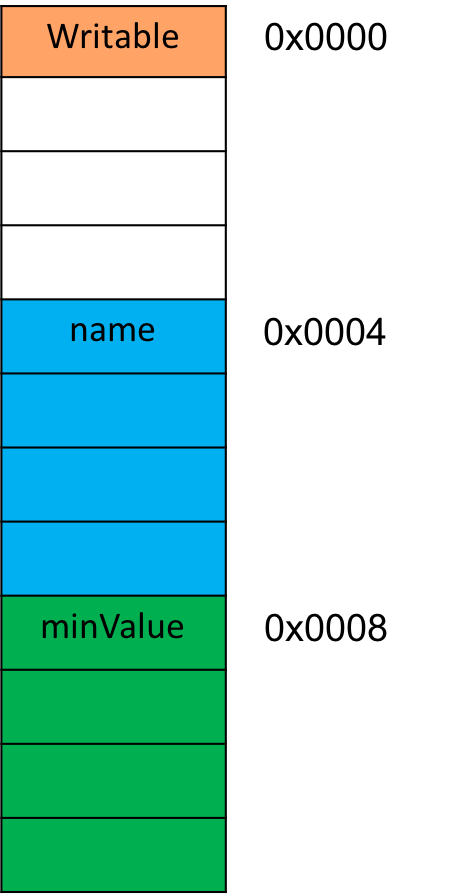
\includegraphics[width=4cm]{Figures/alignement1.png}
\caption{Memory Algnement under 32bits system}
\label{fig:side:a}
\end{minipage}%
\begin{minipage}[t]{0.5\linewidth}
\centering
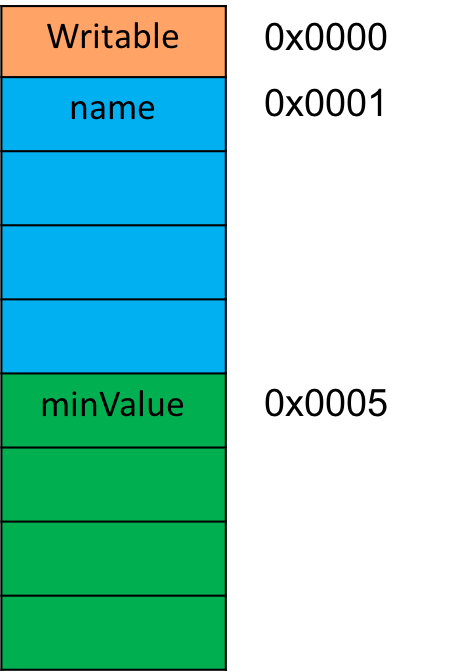
\includegraphics[width=4cm]{Figures/alignement2.png}
\caption{Memory Algnement under 32bits system with packed}
\label{fig:side:b}
\end{minipage}
\end{figure}


Under the Homelive architecture, it can only read data from address that is multiple of 4, so when the program tries to read value of name, the address is 0x0001 which is not an valid address, it reports the \textit{bus error}. To solve this bus error, the easiest way is to delete the attribute \textit{packed}, and then the compilator will automatic shift the address to meet the requirements.

%----------------------------------------------------------------------------------------
\section{RPC methods}
The next step is to verify and implement all the RPC methods, after verification:
\begin{center}
  \begin{tabular}{@{} cc @{}}
    \toprule
    RPC Method & Result \\*
    \midrule
    Connection Request & Yes \\
    Get RPC Methods & Yes \\
    Set Parameter Values  & Yes\\
    Get Parameter Values  & Yes\\
    Set Parameter Attributes  & Yes\\
    Get Parameter Attributes  & Yes\\
    Get Parameter Names & Yes\\
    Add Object  & Yes\\
    Delete Object & Yes\\
    Reboot & No\\
    Downloaded  & Yes\\
    Factory Reset & Yes\\
    Schedule Inform & Yes\\
    Upload & Yes\\
    \bottomrule
  \end{tabular}
%	\caption[Homelive Box of Orange]{Homelive Box of Orange}
\end{center}

When we call \textit{reboot} from ACS, the TR-069 turns out only reboot the program but not the whole box. To repair this, after located the reboot function, we added one line at the end of the function to let the program call the box to reboot after 5 seconds (which is for the TR-069 to shutdown all the process).
\begin{lstlisting}[mathescape]
  /*Reboot system after 5 seconds*/
  system("(sleep 5 && reboot) &");
\end{lstlisting}
 %results
% Chapter 6

\chapter{Discussions} % Main chapter title

\label{Chapter6} % For referencing the chapter elsewhere, use \ref{Chapter6}

\lhead{Chapter 6. \emph{Discussions}} % This is for the header on each page - perhaps a shortened title
The experiments results are interesting and kind of beyond our assumption. 
Firstly, in our assumption, the the MSE loss should be negatively correlated with the number of hidden layer units, but in fact, the MSE loss may oscillated a little and have the tendency but not much. Especially when lambda $\lambda$ become large, it's like hidden layer units number losses its influence on the MSE error. 

Secondly, the result about domain BCE loss seems promising, it's the same for training and for valid. When the lambda $\lambda$ is 0.1, we can see there's little influence about the neural network so the BCE loss is small, means we can still distinguish the session 1 and session 2. but when lambda $\lambda$ become large, the domain BCE loss stay large so that means we have reach our goal (make the representation of the 2 different session become indiscriminate).

Considering the above two parts, for this special subject who provided the EEG data, we should choose a lambda $\lambda$ larger than 10, and the number of hidden layer units should be [10,20] to get the balance between the performance and computation time. %discussion

%----------------------------------------------------------------------------------------
%	THESIS CONTENT - APPENDICES
%----------------------------------------------------------------------------------------

\addtocontents{toc}{\vspace{1em}} % Add a gap in the Contents, for aesthetics

\appendix % Cue to tell LaTeX that the following 'chapters' are Appendices

% Include the appendices of the thesis as separate files from the Appendices folder
% Uncomment the lines as you write the Appendices

% Appendix A

\chapter{Installation of OpenWRT and TR-069} % Main appendix title

\label{AppendixA} % For referencing this appendix elsewhere, use \ref{AppendixA}

\lhead{Appendix A. \emph{Installation of OpenWRT and TR-069}} % This is for the header on each page - perhaps a shortened title

\lstdefinestyle{DOS}
{
    backgroundcolor=\color{black},
    basicstyle=\scriptsize\color{white}\ttfamily
    numbers=none,
    numbersep=8pt,                   % how far the line-numbers are from the code
    numberstyle=\tiny\color{white}, % the style that is used for the line-numbers
    stepnumber=1                    % the step between two line-numbers. If it's 1, each line will be numbered
}
%----------------------------------------------------------------------------------------
\lstdefinestyle{C}
{
  morekeywords={export}
}
%----------------------------------------------------------------------------------------
This appendix will introduce how to getting and building OpenWRT toolchain, compile TR-069 Client and run the client on the Homelive Box.
%----------------------------------------------------------------------------------------
\section{Getting and building OpenWRT toolchain}

\subsection{Get OpenWRT Source}
First to do is create your OpenWRT folder and get the source code of OpenWRT using git or SVN:
\begin{lstlisting}[style=DOS][language=bash]
  $ tsocks svn co -r44360 svn://svn.openwrt.org/openwrt/trunk/ OpenWRT
\end{lstlisting}
or
\begin{lstlisting}[style=DOS][language=bash]
  $ tsocks git clone git://git.openwrt.org/openwrt.git
\end{lstlisting}

We choose the specific version 44360 because OpenWRT added unsupported libraries after this.

\subsection{OpenWRT Buildroot Configuration}
Then is to run configure interface to personalize your OpenWRT image:
\begin{lstlisting}[style=DOS][language=bash]
  $ make menuconfig
\end{lstlisting}

It will show a interface like below:
\begin{figure}[htbp]
	\centering
		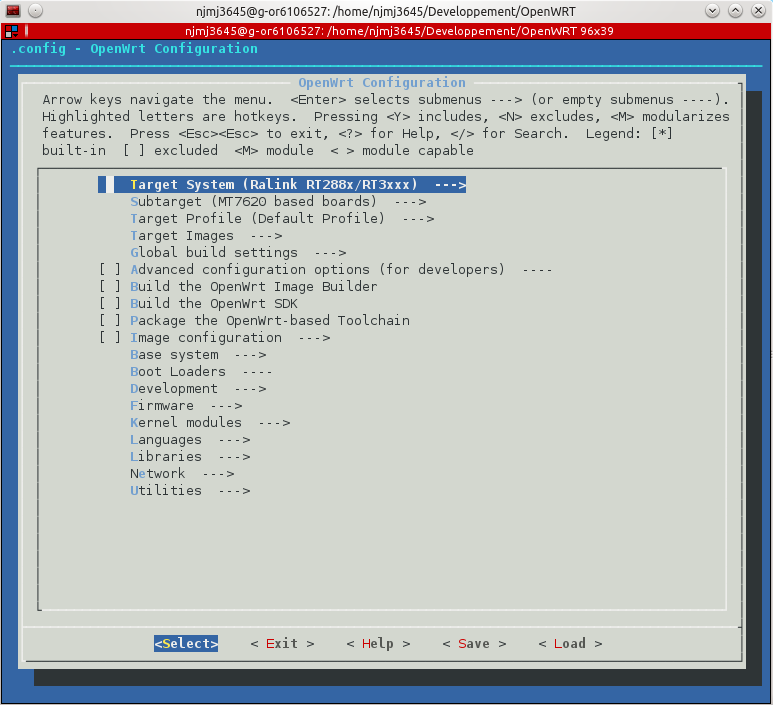
\includegraphics[width=8cm]{Figures/menuconfig.png}
	\caption[OpenWRT Menu Config Interface]{OpenWRT Menu Config Interface}
\end{figure}

\begin{itemize}
  \item In the \textbf{Target System} section, select \textbf{Ralink RT288x/RT3xxx},
  \item In the \textbf{Subtarget} section, select \textbf{MT7620 base boards}.
  \item In the \textbf{Libraries} section, select \textbf{libcurl}.
  \item In the \textbf{Libraries/SSL} section, select \textbf{libopenssl}.
  \item In the \textbf{Base system} section, select \textbf{lipthread}.
\end{itemize}

Then save the new configuration and exit menuconfig.


\subsection{Build the OpenWRT Toolchain}
\begin{lstlisting}[style=DOS][language=bash]
  $ tsocks make
\end{lstlisting}
If there are errors during the compilation. After solving the problem, you can continue the compilation process by using commands like:
\begin{lstlisting}[style=DOS][language=bash]
  $ tsocks make package/install
\end{lstlisting}
or
\begin{lstlisting}[style=DOS][language=bash]
  $ tsocks make package/libs/curl/install
\end{lstlisting}

The compiling process may take a while. When finished, your OpenWRT toolchain is ready to use.

%----------------------------------------------------------------------------------------
\section{Building TR-069 Client}
\subsection{Get the source code}
Getting the source code by using the SVN of Orange:
\begin{lstlisting}[style=DOS][language=bash]
  $ tsocks svn co https://www.forge,orange-labs.fr/svnroot/tr069agent
\end{lstlisting}


Before using OpenWRT toolchain, there are some path to set:
\begin{lstlisting}[style=DOS][language=bash]
  $ export STAGING_DIR=$HOME/path/to/openwrt/staging_dir
  $ export PATH=$PATH:$STAGING_DIR/toolchain-mipsel_24krec+dsp_gcc-4.8-linaro_uClibc-0.9.33.2/bin
\end{lstlisting}

Then, the compiling command is:
\begin{lstlisting}[style=DOS][language=bash]
  $ make Target=HomeLive CC=$STAGING_DIR/toolchain-mipsel_24kec+dsp_gcc-4.8-linaro_uClibc-0.9.33.2/bin/mipsel-openwrt-linux-uclibc-gcc CWMP_APPLICATION_NAME=cwmpd LIB_HEADER_INC=-I$STAGING_DIR/target-mipsel_24kec+dsp_uClibc-0.9.33.2/usr/include/ CWMP_USED_LIBRARY_FLAGS="-L$STAGING_DIR/target-mipsel_24kec+dsp_uClibc-0.9.33.2/usr/lib/ -lcurl -lpthread -lpolarssl -ljsonc"
\end{lstlisting}

You can find exactable file \textit{cwmpd} in ./obj.
%----------------------------------------------------------------------------------------
\section{Connection to the Homelive Box}
\subsection{Port status checking}
First change your network to Livebox LAN. Then use nmap to find the Homelive address:
\begin{lstlisting}[style=DOS][language=bash]
  $ sudo nmap -sP 192.168.1.0/24
\end{lstlisting}
Then check if the Homelive HTTP and SSH port are open:
\begin{lstlisting}[style=DOS][language=bash]
  $ sudo nmap -Pn 192.168.1.10 //Homelive address
  Starting Nmap 6.00 ( http://nmap.org ) at 2015-08-20 10:43 CET
  Nmap scan report for pc5.home (192.168.1.10)
  Host is up (0.0019s latency).
  Not shown: 996 closed ports
  PORT    STATE    SERVICE
  22/tcp  filtered ssh
  53/tcp  open     domain
  80/tcp  filtered http
  443/tcp filtered https

  Nmap done: 1 IP address (1 host up) scanned in 40.73 seconds
\end{lstlisting}

To open the ssh and http port permanently, you can put a script in /root and add the following line to contab:
\begin{lstlisting}[style=DOS][language=bash]
*/2 * * * * /root/permissions.sh >/dev/null 2>&1
\end{lstlisting}
This line will execute the script every 2 minutes.


\subsection{Connect to Homelive}
We will use SSH to connect Homelive box:
\begin{lstlisting}[style=DOS][language=bash]
  $ sudo ssh root@192.168.1.10:/root
\end{lstlisting}
%---------------------------------------------------------------------------------------------------
\section{Running cwmpd on Homelive}
Copy the \textit{cwmpd} bin file and \textit{parameters.csv}, \textit{DeviceInterfaceStubFile} using scp.

\subsection{Library Dependencies}
List of the needed libraries for cwmpd:
\begin{lstlisting}[style=DOS][language=bash]
  $ objdump -p cwmpd | grep NEEDED
  NEEDED               libcurl.so.4
  NEEDED               libpthread.so.0
  NEEDED               libpolarssl.so.7
  NEEDED               libgcc_s.so.1
  NEEDED               libc.so.0
\end{lstlisting}

We need to get the correct version of libpolarssl: libpolarssl.so.3. A temporary hack is to define a symbolic link from libpolarssl.so.7 to libpolarssl.so.3. On the HomeLive:
\begin{lstlisting}[style=DOS][language=bash]
  $ cd /usr/lib
  $ ln -s libpolarssl.so.3 libpolarssl.so.7
  $ ls -l libpolarssl.so*
  lrwxrwxrwx    1 root     root            16 Dec  3 10:49 libpolarssl.so -> libpolarssl.so.3
  -rwxr-xr-x    1 root     root        223675 Feb 21  2014 libpolarssl.so.1.2.9
  lrwxrwxrwx    1 root     root            20 Dec  3 10:49 libpolarssl.so.3 -> libpolarssl.so.1.2.9
  lrwxrwxrwx    1 root     root            16 Jan 13 16:55 libpolarssl.so.7 -> libpolarssl.so.3
\end{lstlisting}


You can run cwmpd using:
\begin{lstlisting}[style=DOS][language=bash]
  $ ./cwmpd -p path/to/parametercsvfile/folder
\end{lstlisting}

\addtocontents{toc}{\vspace{1em}} % Add a gap in the Contents, for aesthetics
% Appendix B

\chapter{JSON parser in C} % Main appendix title

\label{AppendixB} % For referencing this appendix elsewhere, use \ref{AppendixA}

\lhead{Appendix B. \emph{JSON Parser in C}} % This is for the header on each page - perhaps a shortened title
%--------------------------------------------------------------------
\lstdefinestyle{DOS}
{
    backgroundcolor=\color{black},
    basicstyle=\scriptsize\color{white}\ttfamily
    numbers=none,
    numbersep=8pt,                   % how far the line-numbers are from the code
    numberstyle=\tiny\color{white}, % the style that is used for the line-numbers
    stepnumber=1                    % the step between two line-numbers. If it's 1, each line will be numbered
}
%----------------------------------------------------------------------------------------
\lstdefinestyle{C}
{
  morekeywords={export}
}
%----------------------------------------------------------------------------------------
This appendix will explain how to implement the JSON parser in C language using library JSON-c.
%----------------------------------------------------------------------------------------
\section{Objective of JSON Parser}
The objective of our JSON parser is to parser a JSON file generated by Luup HTTP Request. The website \href{http://jsonviewer.stack.hu}{Online JSON Viewer} can be used to visualize the JSON file. Below is a JSON example of our JSON file named \textbf{status.json}:

\begin{figure}[htbp]
	\centering
		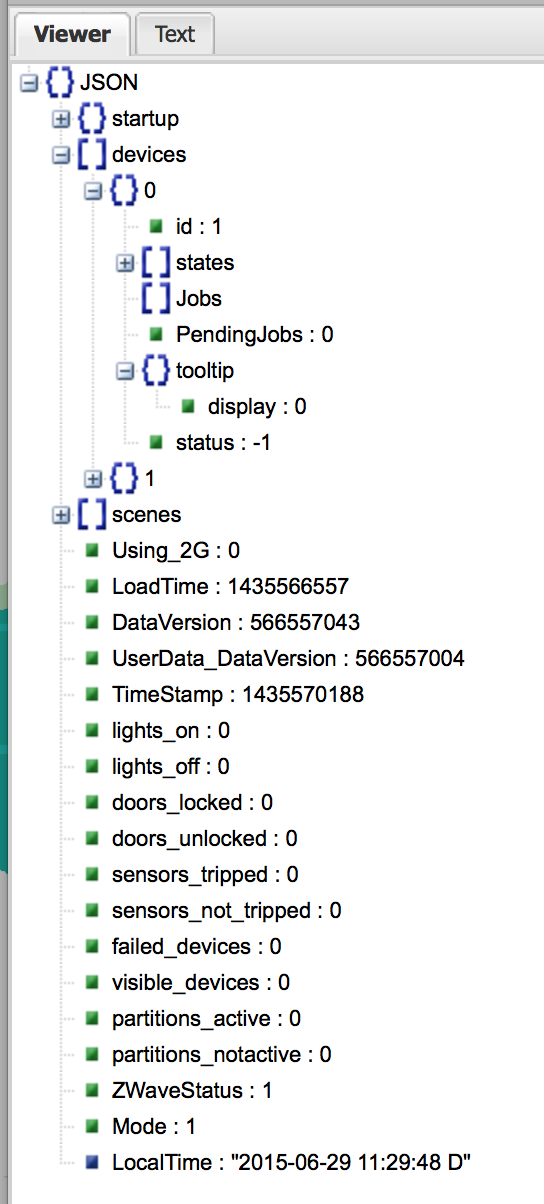
\includegraphics[width=5cm]{Figures/jsonviewer.png}
	\caption[JSON File in JSON Viewer Online]{JSON File in JSON Viewer Online}
\end{figure}

In order to import the data into TR-069, the JSON format should be convert to Z-Wave format which is like:
\begin{lstlisting}[mathescape]
    ZWave.devices.1.id 1
    ZWave.devices.1.states.1.id 208
    ZWave.devices.1.states.1.service urn:micasaverde-com:serviceId:ZWaveNetwork1
    ZWave.devices.1.states.1.value 1
    ZWave.devices.1.states.2.id 209
    ZWave.devices.1.states.2.service urn:micasaverde-com:serviceId:ZWaveNetwork1
    ZWave.devices.1.states.2.variable UseMR
    ZWave.devices.1.states.2.value 1
    ZWave.devices.1.states.3.id 210
    ZWave.devices.1.states.3.service urn:micasaverde-com:serviceId:ZWaveNetwork1
    ZWave.devices.1.states.3.variable LimitNeighbors
    ZWave.devices.1.states.3.value 0
    ZWave.devices.1.states.4.id 211
    ZWave.devices.1.states.4.service urn:micasaverde-com:serviceId:ZWaveNetwork1
    ZWave.devices.1.states.4.variable LastDongleBackup
\end{lstlisting}

First part is the name and second is the value.
%----------------------------------------------------------------------------------------------
\section{JSON Format Characteristic}
JSON is built on two structures:

\begin{itemize}
  \item A collection of name/value pairs. In various languages, this is realized as an object, record, struct, dictionary, hash table, keyed list, or associative array.
  \item An ordered list of values. In most languages, this is realized as an array, vector, list, or sequence.
\end{itemize}
An object is an unordered set of name/value pairs. An object begins with \{ (left brace) and ends with \} (right brace). Each name is followed by: (colon) and the name/value pairs are separated by, (comma).

\begin{figure}[htbp]
	\centering
		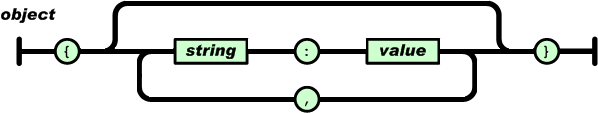
\includegraphics[width=12cm]{Figures/jsonobject.png}
	\caption[JSON Object Structure]{JSON Object Structure}
\end{figure}

An array is an ordered collection of values. An array begins with [ (left bracket) and ends with] (right bracket). Values are separated by, (comma).
\begin{figure}[htbp]
	\centering
		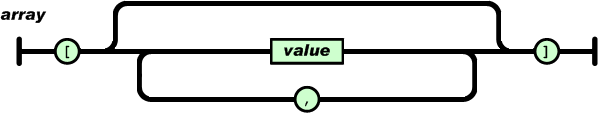
\includegraphics[width=12cm]{Figures/jsonarray.png}
	\caption[JSON Array Structure]{JSON Array Structure}
\end{figure}

In the array case, the index must be added after the last level (e.g. ZWave.devices.1.states.2.id 209). The parser works in an iterative way.

\section{Implementation of JSON Parser}

At first, we set a buffer to store the path for each parameter. Then use the json-c library function \textit{json\_object\_from\_file} to save all the file content into a JSON object:

\begin{lstlisting}[mathescape]
    char path_json[70] = "ZWave.";    //set the buffer to save the name of parameter, also as the head

    struct json_object* jobj = json_object_from_file(fichierLu);  //fichierLu set to the file path to parse

    _jsonParser(path_json, jobj);  //jobj is the json object will be parsed
\end{lstlisting}


\textit{\_jsonParser} is the private function to parse the JSON object. There is a essential json-c library function called \textit{json\_object\_object\_foreach(jobj, key, val)}, it allows to traverse each object in the JSON object. Before that, the current path should be added into a string.

\begin{lstlisting}[mathescape]
    /*Parsing the json object*/
    void _jsonParser(char *path, json_object * jobj)
    {
       enum json_type type;

       char parse_path[100];                          //define the local variable for path
       strcpy(parse_path,path);

       json_object_object_foreach(jobj, key, val)   /*Passing through every array element*/
       {
          type = json_object_get_type(val);
          switch (type)
          {
             case json_type_boolean:
             case json_type_double:
             case json_type_int:
             case json_type_string:  _printJsonValue(parse_path, val, key);
                                     break;

             case json_type_object:  sprintf(&parse_path[strlen(parse_path)], "%s.",key );
                                     jobj = json_object_object_get(jobj, key);
                                     _jsonParser(parse_path, jobj);
                                     break;

             case json_type_array:   _jsonParseArray(jobj, key, parse_path);
                                     break;
          }
       }
    }
\end{lstlisting}

If the object parsed is a value, jump to the \textit{\_printJsonValue} function to save the value in buffer table. If it's a object, redo this function. If it's an array, go to the \textit{\_jsonParseArray} function.

\begin{lstlisting}[mathescape]
    /*Parsing the json array*/
    void _jsonParseArray( json_object *jobj, char *key, char *path)
    {
       void _jsonParser(char *path, json_object * jobj); /*Forward Declaration*/
       enum json_type type;

       char array_path[100];                            //define the local variable for path
       strcpy(array_path,path);
       json_object * jvalue;


       json_object *jarray = jobj; /*Simply get the array*/

       if(key) {jarray = json_object_object_get(jobj, key); /*Getting the array if it is a key value pair*/}

       int arraylen = json_object_array_length(jarray); /*Getting the length of the array*/
       int i;

       sprintf(&array_path[strlen(array_path)],"%s.",key);

       sprintf(&array_path[strlen(array_path)],"x.");   //fill the path with x. for instance

       for (i=0; i< arraylen; i++)
       {
          jvalue = json_object_array_get_idx(jarray, i); /*Getting the array element at position i*/
          type = json_object_get_type(jvalue);

          if( i <= 9 )
             sprintf(&array_path[strlen(array_path)-2], "%d.",i + 1 );  //replace the 2 last char x.
          else
             sprintf(&array_path[strlen(array_path)-3], "%d.",i + 1 );  //replace the 3 last char xx.


          if (type == json_type_array)
             _jsonParseArray(jvalue, NULL,array_path);
          else if (type == json_type_object)
             _jsonParser(array_path, jvalue);
          else
             _printJsonValue(array_path, jvalue, NULL);
       }
    }
\end{lstlisting}

The main difficulty of parse a array is to add the index. The solution is to add .x at every beginning of Array parse, and then replace the .x according to different object type.

\begin{lstlisting}[mathescape]
    /*At the end of each iteration, write the name/value pair to a 2D table*/
    void _printJsonValue( char* path, json_object *jobj, char *key)
    {
      enum json_type type;

      type = json_object_get_type(jobj); /*Getting the type of the json object*/

      char* value_buffer;
      value_buffer = (char*)malloc(150 * sizeof(char));

      char* paramKey;
      paramKey = (char*)malloc((strlen(path)+strlen(key)) * sizeof(char));

      strcpy(paramKey,path);         //build the JSON object name string
      strcat(paramKey,key);

      switch (type)
      {
          case json_type_boolean: sprintf(value_buffer,"%s",json_object_get_boolean(jobj)? "true": "false");
                                  sdataParameterList[indiceValueStruct] = DM_ENG_newSystemParameterValueStruct(paramKey, value_buffer, NULL);
                                  break;
          case json_type_double:  sprintf(value_buffer,"%lf",json_object_get_double(jobj));
                                  sdataParameterList[indiceValueStruct] = DM_ENG_newSystemParameterValueStruct(paramKey, value_buffer, NULL);
                                  break;
          case json_type_int:     sprintf(value_buffer,"%d",json_object_get_int(jobj));
                                  sdataParameterList[indiceValueStruct] = DM_ENG_newSystemParameterValueStruct(paramKey, value_buffer, NULL);
                                  break;
          case json_type_string:  value_buffer = strdup(json_object_get_string(jobj));
                                  sdataParameterList[indiceValueStruct] = DM_ENG_newSystemParameterValueStruct(paramKey, value_buffer, NULL);
                                  break;
      }
      free(value_buffer);
      indiceValueStruct++;
    }
\end{lstlisting}

On the \textit{\_printJsonValue} function, each element in the buffe table is a TR-069 \textit{System Parameter Value Struct} using the TR-069 Client API default function \textit{DM\_ENG\_newSystemParameterValueStruct}.

\addtocontents{toc}{\vspace{1em}} % Add a gap in the Contents, for aesthetics
%\input{Appendices/AppendixC}

%\addtocontents{toc}{\vspace{1em}} % Add a gap in the Contents, for aesthetics

\backmatter

%----------------------------------------------------------------------------------------
%	BIBLIOGRAPHY
%----------------------------------------------------------------------------------------

\label{Bibliography}

\lhead{\emph{Bibliography}} % Change the page header to say "Bibliography"

\bibliographystyle{unsrtnat} % Use the "unsrtnat" BibTeX style for formatting the Bibliography

\bibliography{Bibliography} % The references (bibliography) information are stored in the file named "Bibliography.bib"

\addtocontents{toc}{\vspace{1em}} % Add a gap in the Contents, for aesthetics
%
%%----------------------------------------------------------------------------------------
%%	ABSTRACT PAGE
%%----------------------------------------------------------------------------------------
%\setstretch{1.5} % Reset the line-spacing to 1.5 for body text (if it has changed)
%
%\clearpage % Start a new page
%
%\frontmatter % Use roman page numbering style (i, ii, iii, iv...) for the pre-content pages
%
%\abs{\addtocontents{toc}{\vspace{1em}} % Add a gap in the Contents, for aesthetics
%
%The TR-069 developed by Orange Labs allows to manage communication between customer-premises equipment (CPE) and Auto Configuration Server (ACS).It offers the use of a set of services administration, monitoring and diagnosis while avoiding the problems associated with hardware and software diversity.
%
%Orange Homelive is the solution to manage the home on the mobile. From a single application, Homelive allows to interact with connected compatiable objects in the house. It proposes the Smart Home solution with a set-top box--Homelive.
%
%Z-Wave is a wireless protocol designed for home automation (lighting, private heating) and so-called Smart Home. Z-Wave was bought by the company Americane Sigma Designs in 2008. It is optimized for low bandwidth exchanges and devices on battery. It can be easily integrated in consumer electronics, including remote controls, smoke detectors and safety sensors.
%
%During the six-month internship, my main mission was to adapt the TR-069 Client at the Homelive box by resolving the incompatibility and implementing the RPC methods. Also, integrates the new Z-Wave data model in the TR-069 Client by contacting with the Luup firmware of the Homelive Box. With my internship result, Orange will be allowed to manage Homelive from distance to reduce the expenses on support services.
%}
%
%%----------------------------------------------------------------------------------------
%	RÉSUMÉ PAGE
%----------------------------------------------------------------------------------------
%
%\clearpage % Start a new page
%
%\resume{\addtocontents{toc}{\vspace{1em}} % Add a gap in the Contents, for aesthetics
%
%Le TR-069 développé par Orange Labs permet de gérer la communication entre un équipement terminal du réseau local du client et un servert d'autoconfiguration associé dans un même réseau apprtenant à l'opérateur.Il offre à l'utilisation d'un ensemble de services d'administration, de contrôle et de diagnostic tout en évitant les problèmes liés aux diversités matérielles et logicielles.
%
%Orange Homelive est la solution pour piloter sa maison depuis son mobile. A partir d'une seule application, Homelive permet d'interagir avec les objets connectés compatiables dans la maison. Il donne la solution de Smart Home avec un set-top box--Homelive.
%
%Z-Wave est un protocole radio conçu pour la domotique(éclairage, chauffrage) et ce qu'on appelle l'Habitat comminicant. En 2008 Z-Wave a été rachetée par la société américane Sigma Designs. Il est optimisé pour des échanges à faible bande passante et des appareils sur pile ou alimentés électroniquement. Il peut être facilement intégrée dans les produits électroniques de consommation, y compris télécommandes, les détecteurs de fumée et capteurs de sécurité.
%
%Pendant ces six mois de stage, ma mission principale a été d'adapter le TR-069 Client au Homelive box, en résoulvant les incompatibilité et implémentant les RPC méthodes. Ainsi que intégre le nouveau data modèle Z-Wave dans le TR-069 Client en communiquant avec le firmware Luup dans Homelive Box. Avec mon résultat de stage, Orange va être autorisé à gérer Homelive à distance pour réduire les dépenses sur les services de soutien.
%}

%----------------------------------------------------------------------------------------
\end{document}
